\documentclass{article}
\usepackage[T1]{fontenc}
\usepackage{amsmath}
\usepackage[parfill]{parskip}
\usepackage{lipsum}
\usepackage{bm}
\usepackage{microtype}
\usepackage{listings}
\usepackage{graphicx}
\usepackage{setspace}
\usepackage[norsk]{babel}
\graphicspath{ {./figurer/} }

\title{Obligatorisk oppgave 1 - IN2090}
\author{Oscar Atle Brovold}
\date{12. sep - 27. sep}

\begin{document}
\onehalfspacing

\begin{titlepage} % Oppretter en separat tittelside
    \centering
    \vspace*{5cm} % Vertikal plass før tittelen, juster etter behov
    {\Huge \bfseries Obligatorisk oppgave 1 \ IN2090\par}
    \vspace{1.5cm}
    {\Large Oscar Atle Brovold\par}
    \vspace{1.5cm}
    {\Large 12. sep - 27. sep\par} % Dato, kan endres til fast dato
    \vfill
\end{titlepage}

\newpage % Tvinger ny side før selve oppgaven begynner

\section*{Oppgave 1 - Fremmed kommunikasjon}
ER-diagrammet i figur \ref{fig:oppgave1} har to entiteter:\
\begin{itemize}
    \item YMLE
    \item BAMLE
\end{itemize}
Entiteter har verdier knytttet til seg, kjent som attributer, ER-diagrammet i figur \ref{fig:oppgave1}
har to attributer knyttet til YMLE og en attribut knyttet til BAMLE. 
\begin{itemize}
    \item YMLE
    \begin{enumerate}
        \item Gru
        \item Blipp 
    \end{enumerate}
    \item BAMLE
    \begin{enumerate}
        \item Blunk
    \end{enumerate}
\end{itemize}

En strek under ordet betyr at attributten er unik, dette er kjent som nøkler. YMLE sin nøkkel er
Blipp og BAMLE sin nøkkel en Blunk. 

Til slutt har vi en relasjon, relasjoner relaterer to eller flere entiteter. I figur \ref{fig:oppgave1}
relateres YMLE og BAMLE gjennom relasjonen ZLUFF. N til venstre for ZLUFF
i kombinasjon med dobbel linje betyr at BAMLE ZLUFFer opptil N YMLEer med minimum en, og 1 til høyre 
i kombinasjon med enkel linje betyr at YMLE ZLUFFer maks en og minst null BAMLEer.

\begin{figure}[h!]
    \centering
    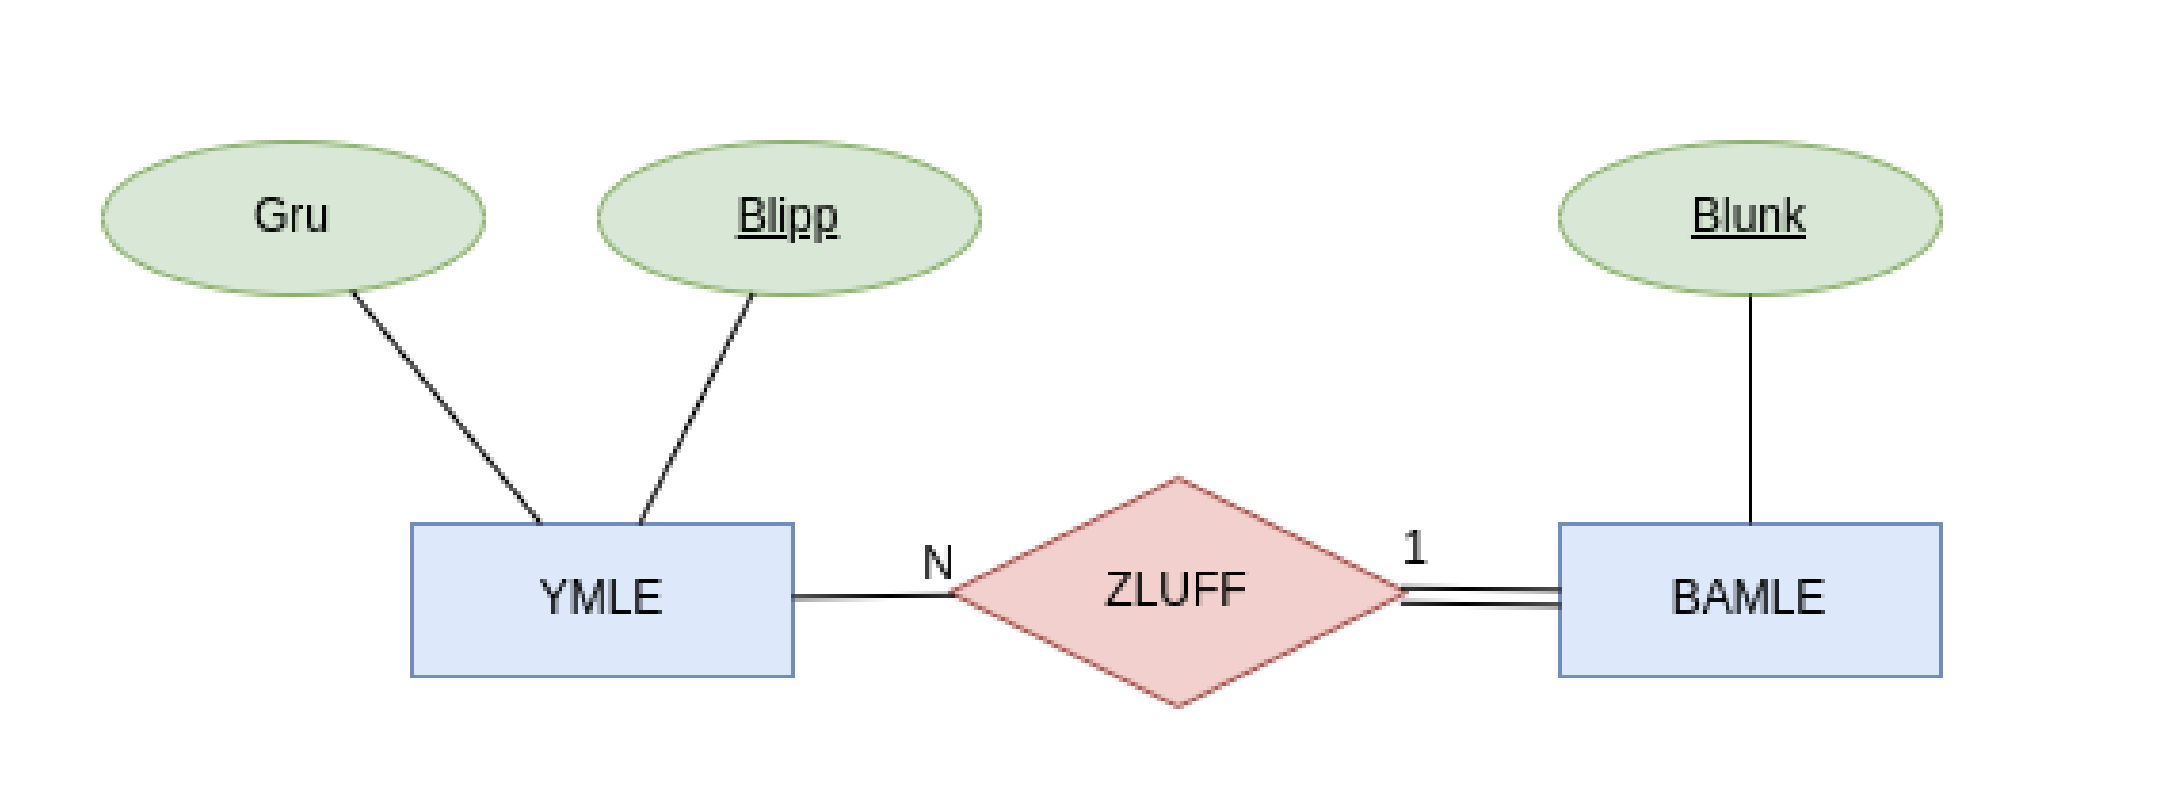
\includegraphics[width=1\textwidth]{oppgave1} % Replace with your image file
    \caption{ER-diagram som skal forklares i oppgave 1} % Add your caption text here
    \label{fig:oppgave1} % Optional: label for referencing the figure
\end{figure}
\newpage
\section*{Oppgave 2 – Menneskelig Svar}
% Oppgaveteksten gir følgende ER-diagram:
\begin{figure}[h!]
    \centering
    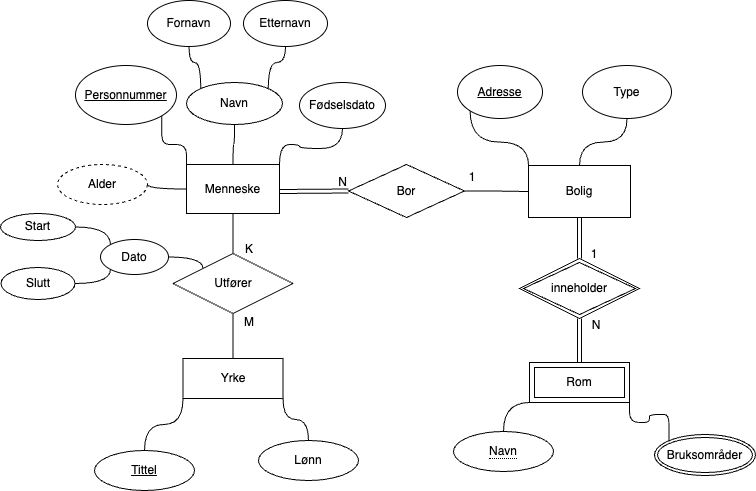
\includegraphics[width=0.9\textwidth]{oppgave2_oblig1.png} % Replace with your image file
    \caption{ER-diagram for menneskelig svar oppgave 2} % Add your caption text here
    \label{fig:oppgave2} % Optional: label for referencing the figure
\end{figure}

\section*{Oppgave 3 - Romvesnene}
% Oppgaveteksten gir følgende ER-diagram:
\begin{figure}[h!]
    \centering
    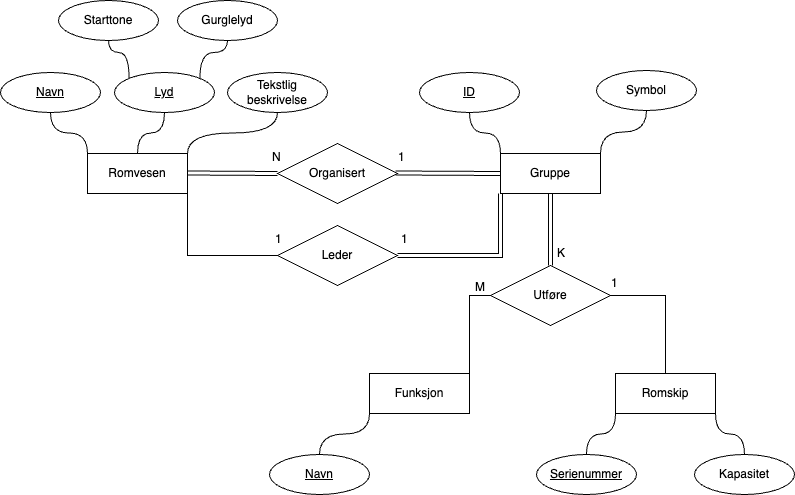
\includegraphics[width=0.9\textwidth]{oppgave3_oblig1.png} % Replace with your image file
    \caption{ER-diagram for romvesnene oppgave 3} % Add your caption text here
    \label{fig:oppgave3} % Optional: label for referencing the figure
\end{figure}

\section*{Oppgave 4 - Lagre kommunikasjon}
\subsubsection*{Mulig realisering av ER-diagrammet i figur \ref{fig:oppgave4}}
Menneske(brukernavn, personnr., navn) \\
\begin{tabular}{l l l}
    - KN: & \{brukernavn\}, \{personnr.\} \\
    - PN: & \{personnr.\} \\
\end{tabular}\\
\\
Romvesen(navn, gruppe)\\
\begin{tabular}{l l l}    
    - KN/PN: & \{navn\} \\ 
\end{tabular}\\
\\
Melding(ID, diagram, dato, klokkeslett, mn\_mottaker) \\
\begin{tabular}{l l l}
    - KN/PN: & \{ID\} \\
    - FN: & (mn\_mottaker) \(\rightarrow\) Mennekse(personnr.)\\
\end{tabular}\\
\\
Vedlegg(navn, innhold, ID)\\
\begin{tabular}{l l l}
    - KN/PN: & \{navn, ID\}\\
    - FN: & (ID) \(\rightarrow\) Melding(ID)\\
\end{tabular}\\
\\
RV\_MOTTAKER(ID, navn)\\
\begin{tabular}{l l l}
    - KN/PN: & \{ID, navn\}\\
    - FN: & (ID)   & \(\rightarrow\) Melding(ID) \\
          & (navn) & \(\rightarrow\) Romvesen(navn) \\
\end{tabular}\\
\\
Ansvarsområde(personnr., ansvarsområde)\\
\begin{tabular}{l l l}
   - KN/PN: & \{personnr., ansvarsområde\} \\
   - FN: & (personnr.)  \(\rightarrow\) Menneske(personnr.)\\
\end{tabular} \\
\subsubsection*{Valg som har blitt gjort under realisering}
\textbf{-Realisering av normale entiteter}

\begin{itemize}
    \item \textbf{Mennekse}: Velger personnr. som kandidatnøkkel. Dette er et tilfeldig valg. Aventer med flerverdi attributter.
    \item \textbf{Romvesen} og \textbf{melding}: Kan kun representeres på en måte. 
\end{itemize}

\textbf{-Realisering av svake entiteter}
\begin{itemize}
    \item \textbf{Vedlegg}: Ignorerer utledbare attributter.
\end{itemize}
\newpage
\textbf{-Realisering av 1 til N relasjoner}
\begin{itemize}
    \item \textbf{MN\_MOTTAKER}: To valg, \(i\) ny relasjon eller \(ii\) legge fremmednøkkel inn i N-siden. \
    Velger \(ii\), dette minimerer antall relasjoner. 
\end{itemize}

\textbf{-Realisering av N til M relasjoner}
\begin{itemize}
    \item \textbf{RV\_MOTTAKER}: Kun et valg, må opprette ny relasjon.
\end{itemize}

\textbf{-Realisering av flerverdi-attributter}
\begin{itemize}
    \item \textbf{Ansvarsområde:} Kun et valg, blir egen relasjon.  
\end{itemize}

\begin{figure}[h!]
    \centering
    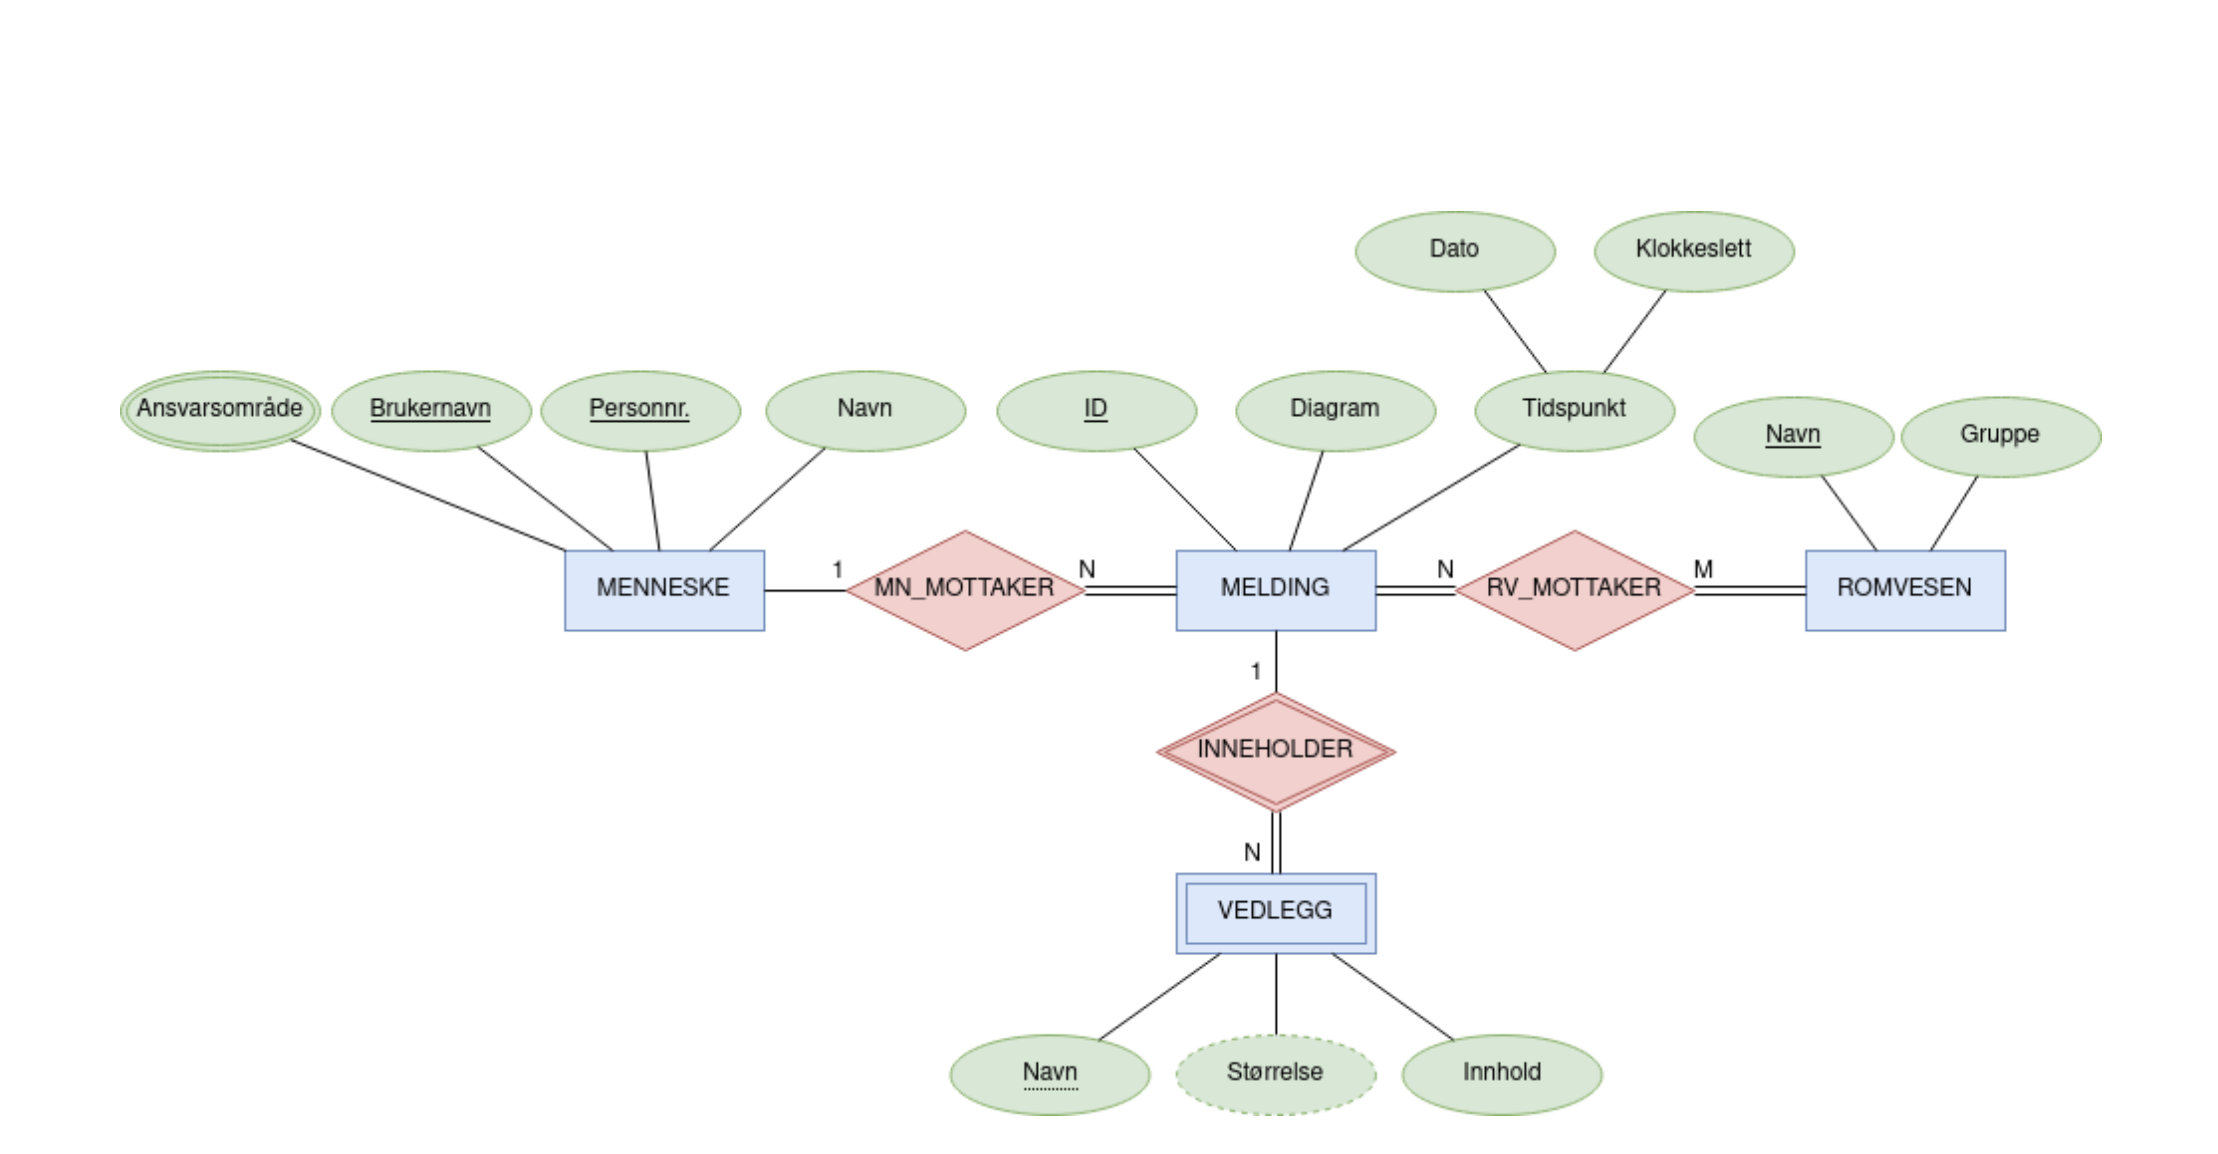
\includegraphics[width=1\textwidth]{oppgave4.png} % Replace with your image file
    \caption{Gitt ER-diagram som skal realiseres i oppgave 4} % Add your caption text here
    \label{fig:oppgave4} % Optional: label for referencing the figure
\end{figure}
\hfill
\begin{center}
\textbf{--- Slutt på obligatorisk oppgave 1 ---}
\end{center}

\end{document}
